\chapter{Einbinden von Grafiken, Sourcecode und Anforderungen}
\label{Kap3}

\section{Bilder}

Natürlich können auch Grafiken und Bilder eingebunden werden, siehe z.\,B. Abbildung~\ref{Kap2:NasaRover}.

\begin{figure}[ht]
  \centering
  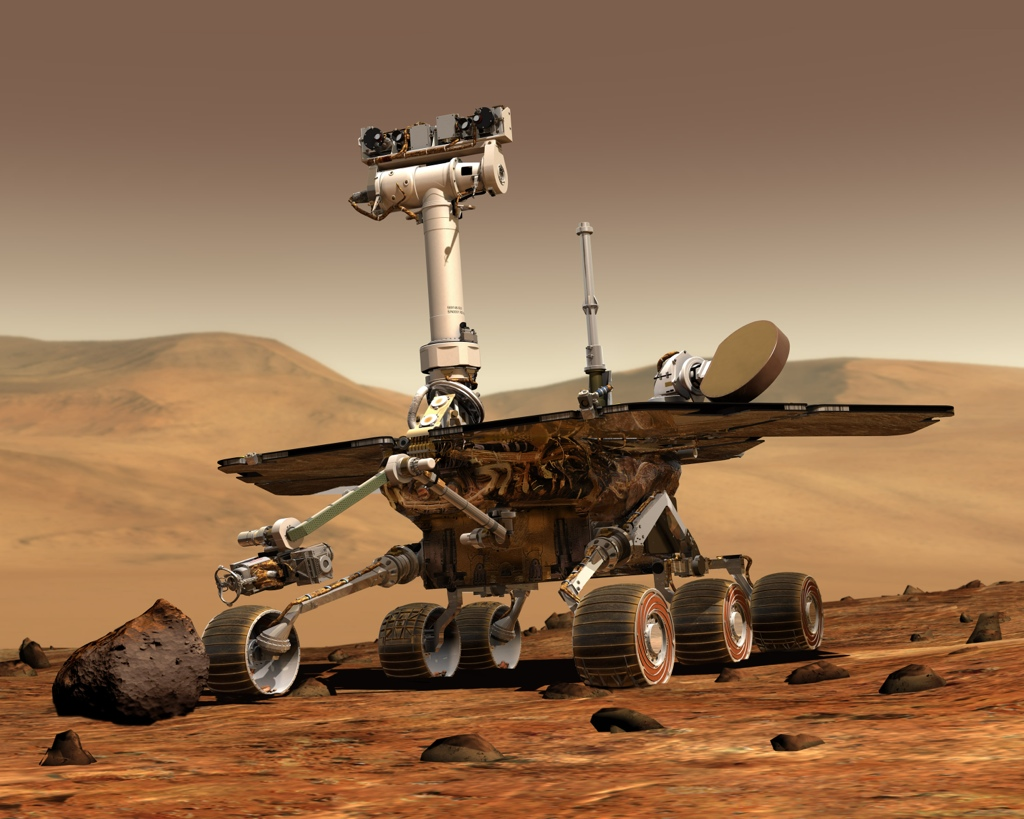
\includegraphics[width=6cm]{images/nasa_rover}
  \caption{Ein Nasa Rover}
  \label{Kap2:NasaRover}
\end{figure}

Man kann sich auch selbst ein Makro für das Einfügen von Bildern schreiben:

\bild{images/modell_point_to_point}{6cm}{Point to Point}

\begin{sidewaysfigure}
 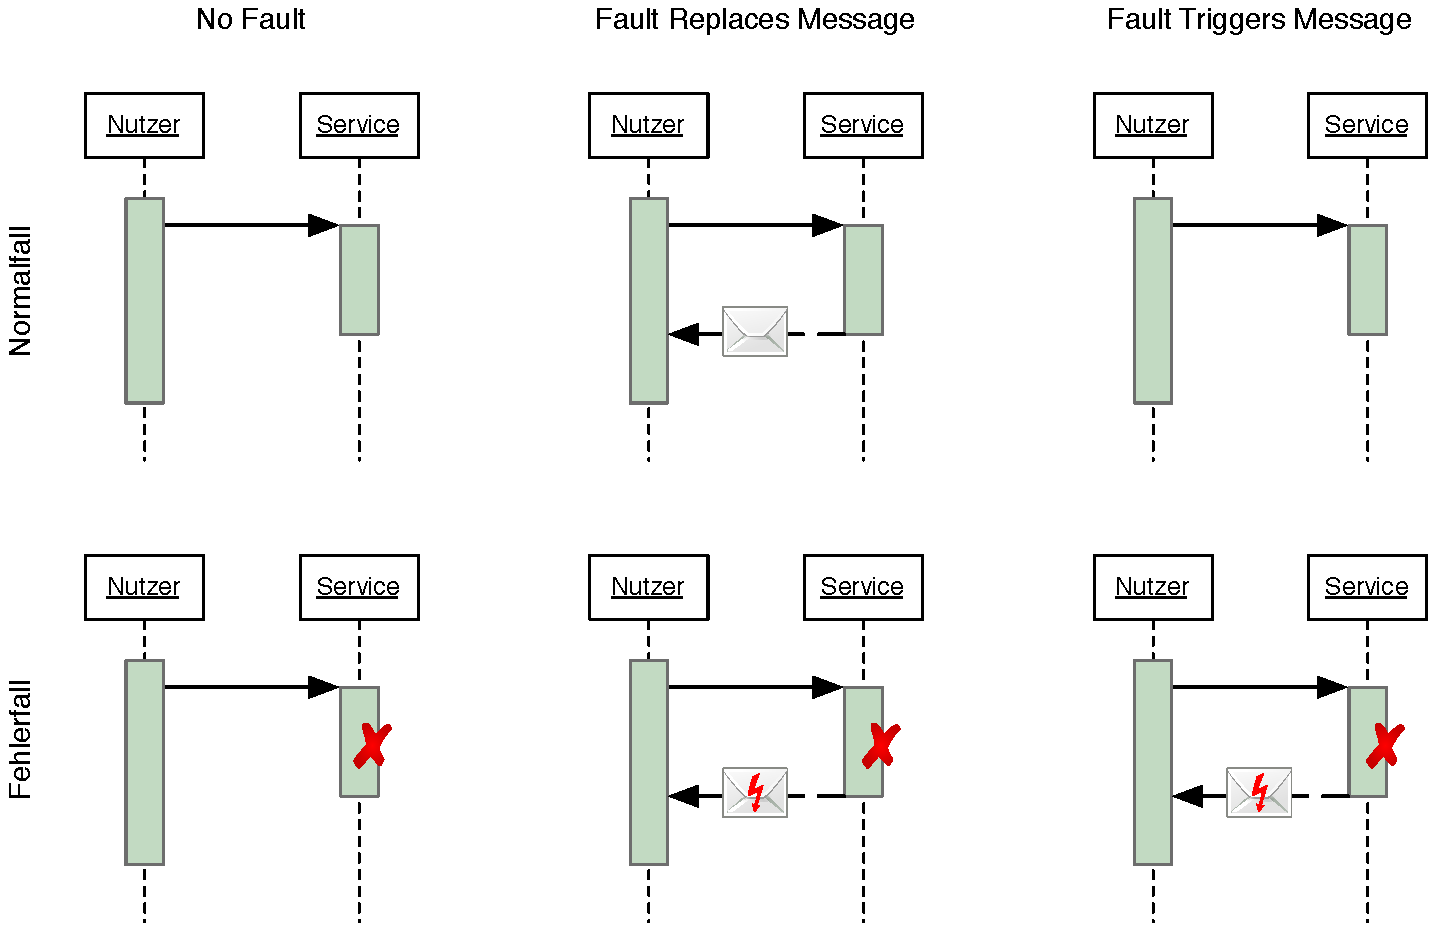
\includegraphics[width=22cm]{images/ws-wsdl20-fehler}
  \caption{Sehr große Grafiken kann man drehen, damit sie auf die Seite passen}
  \label{Kap2:wsdl-fehler}
\end{sidewaysfigure}

\clearpage % Alle Bilder, die bisher kamen ausgeben


\section{Formelsatz}

Eine Formel gefällig? Mitten im Text $a_2 = \sqrt{x^3}$ oder als eigener Absatz (siehe Formel~\ref{Formel}):

\begin{equation}
\begin{bmatrix}
   1 &  4 &  2 \\
   4 &  0 & -3
\end{bmatrix}
        \cdot
\begin{bmatrix}
   1 &  1 &  0 \\
  -2 &  3 &  5 \\
   0 &  1 &  4
\end{bmatrix}
       {=}
\begin{bmatrix}
  -7 &  15 &  28 \\
   4 &   1 & -12
\end{bmatrix}
\label{Formel}
\end{equation}


\section{Sourcecode}

Man kann mit Latex auch ganz toll Sourcecode in den Text aufnehmen.

\subsection{Aus einer Datei}

\lstinputlisting[firstline=2,language=Java,caption={Crypter-Interface},label=lst:CrypterInterface]{\sourcecode/Crypter.java}


\subsection{Inline}

\begin{lstlisting}[language=Java,caption=Methode checkKey()]
    /**
     * Testet den Schlüssel auf Korrektheit: Er muss mindestens die Länge 1
     * haben und darf nur Zeichen von A-Z enthalten.
     *
     * @param key zu testender Schlüssel
     * @throws CrypterException wenn der Schlüssel nicht OK ist.
     */
    protected void checkKey(Key key) throws CrypterException {

        // Passt die Länge?
        if (key.getKey().length == 0) {
            throw new CrypterException("Der Schlüssel muss mindestens " +
                    "ein Zeichen lang sein");
        }

        checkCharacters(key.getKey(), ALPHABET);
    }
\end{lstlisting}


\section{Anforderungen}

Anforderungen im Format des Volere"=Templates (Snowcards) \autocite{Volere} können per Makro eingefügt werden. Das Label wird automatisch mit der Nummer erstellt, d.\,h. Sie können auf die Tabelle mit dieser referenzieren (siehe \autoref{F52}).

Die Abgrenzung von funktionalen und nicht-funktionalen Anforderungen ist nicht immer einfach und bereitet manchen Studierenden Probleme. Als Hilfestellung kann die von der ISO25010 \autocite{ISO25010} zur Verfügung gestellte Liste dienen, siehe \autoref{kapitel3/iso25010}.

\bild{images/iso25010}{14cm}{Qualitätsmodell für Software-Produkte nach ISO25010}

\citeauthor{Bass2003} listen in \autocite{Bass2003} eine ähnliche Liste von Kategorien für nicht-funktionalen Anforderungen auf, die ebenfalls als Richtschnur dienen kann. Diese sind:

\begin{itemize}
  \item \textit{Verfügbarkeit} \textit{(availability)} -- umfasst Zuverlässigkeit (reliability), Robustheit (robustness), Fehlertoleranz (fault tolerance) und Skalierbarkeit (scalability)
  \item \textit{Anpassbarkeit} \textit{(modifiability)}, umfasst Wartbarkeit (maintainability), Verständlichkeit (understandability) und Portabilität (portability).
  \item \textit{Performanz} \textit{(performance)}
  \item \textit{Sicherheit} \textit{(security)}
  \item \textit{Testbarkeit} \textit{(testability)}
  \item \textit{Bedienbarkeit} \textit{(usability)}
\end{itemize}
